
\newcommand{\dlink}[3]{\href{#1}{$\Delta^{#2}\sb{#3}$}}

\spis{Do powierzchni obrotowych i~jeszcze~dalej}
{Michał Miśkiewicz}
\label{Tytul}
\wtyt{\hspace*{-5.5cm}Do powierzchni obrotowych i~jeszcze dalej}
\waut{Michał MIŚKIEWICZ*}
\aafil{Wydział Matematyki, Informatyki i~Mechaniki, Uniwersytet Warszawski}

\vspace{-5mm}
\setlength{\epigraphwidth}{0.5\textwidth}
\epigraph{Full ahead, mr. Sulu, maximum warp.\vspace*{-5pt}}{\vrule height9pt width0ptJames T. Kirk, \\[1mm]\scriptsize\emph{Star Trek: The Original Series}, S01E08} 
\vspace{-1mm}
%\note{\href{https://getyarn.io/yarn-clip/e3bb80cf-cb1c-4d96-8282-370d0475b348}{\emph{Full ahead, mr. Sulu, maximum warp}}. Niestety, \emph{prędkość warp} to słabe tłumaczenie, bo \emph{maximum} odnosi się do maksymalnego \emph{warp factor}. Należałoby sprawdzić w jakichś napisach do Star Treka, co tam powinno być.}

Bohaterem tego artykułu jest \emph{produkt skręcony}, po angielsku: \emph{warped product}. Słowo \emph{warp} (wykrzywić, odkształcić) zrobiło karierę za sprawą \emph{warp drive}, hipotetycznego napędu pozwalającego rozwijać prędkości nadświetlne.  Został on spopularyzowany w~serii science fiction Star Trek i~doczekał się całkiem poważnego traktowania, o~czym więcej można przeczytać w~\emph{Opowieściach o~podróżach w~kosmos} z~\dlink{https://www.deltami.edu.pl/2013/05/opowiesci-o-podrozach-w-kosmos/}{5}{13}, lub też wyszukując hasło \emph{Alcubierre drive}. 
\marg{
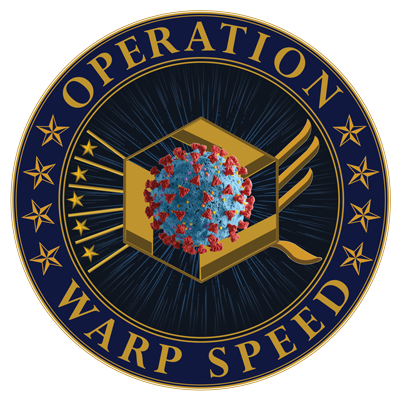
\includegraphics[width=40mm]{ilustracje/Operation_Warp_Speed.png} \\
Oficjalne logo \emph{Operation Warp Speed}, partnerstwa publiczno-prywatnego mającego na celu szybki rozwój i~dystrybucję szczepionek przeciwko covid-19 (maj 2020 -- luty 2021). 
}
Wpływ tej idei na zbiorową wyobraźnię jest na tyle duży, że w~2020 roku amerykańska inicjatywa rozwoju i~dystrybucji szczepionek przeciwko covid-19 przyjęła nazwę \emph{Operation Warp Speed}. 

Nazwa nie jest jedyną cechą łączącą produkt skręcony z~napędem warp. Po pierwsze, napęd ten opiera się na pomyśle odkształcania przestrzeni, co rodzi pojęciową trudność: wszak umiemy giąć dwuwymiarową kartkę w~trójwymiarowej przestrzeni, ale jak mielibyśmy wyginać samą przestrzeń? Odpowiedzią na tę trudność jest geometria wewnętrzna, czyli język pozwalający opisywać geometrię i~deformacje obiektu samego w~sobie, bez odwołań do otaczającej go przestrzeni. Produkt skręcony jest właśnie jednym z~narzędzi takiego opisu. 

Po drugie, przekroczenie prędkości światła konwencjonalnymi metodami nie jest możliwe. Furtkę do obejścia tego zakazu proponuje napęd warp. Ograniczenie ,,prędkości'' podobnej natury zobaczymy niżej, badając bliżej powierzchnie obrotowe. Przekonamy się, że produkt skręcony umożliwia pokonanie tej granicy. Zachęcam więc Czytelnika do lektury, by \emph{odkrywać dziwne nowe światy} oraz \emph{śmiało pójść tam, gdzie żaden człowiek wcześniej nie dotarł}. 
%Kapitan Kirk byłby dumny. 
%\nnote{Tłumaczenie własne według Wikipedii (\href{https://en.wikipedia.org/wiki/Where_no_man_has_gone_before}{link}). Warto się rozejrzeć za jakimś oficjalnym tłumaczeniem.} 

\styt{Powierzchnie obrotowe.} Przepis na taką powierzchnię jest prosty. 
\marg[-60]{
\begin{tikzpicture}
  \draw[-latex](-1,0)--(1.3,0);
  \draw[-latex](0,-.8)--(0,.8);
  \draw[black!20](0,0) ellipse (.25 and .4);
  \draw[black!20](-.8,0) ellipse (.25 and .4);
  \draw[black!20](.8,0) ellipse (.25 and .4);
  \draw[magenta, very thick](-.8,.4)--(.8,.4);
  \draw[black!20](-.8,-.4)--(.8,-.4);
\end{tikzpicture}\quad
\begin{tikzpicture}
  \draw[-latex](-1,0)--(1.3,0);
  \draw[-latex](0,-.8)--(0,.8);\draw[magenta, very thick]	
	plot[samples=20,domain=-1:1]
	(\x, {sqrt(\x*\x+1)-.84});
  \draw[-latex](0,-.8)--(0,.8);\draw[black!20]	
	plot[samples=20,domain=-1:1]
	(\x, {-sqrt(\x*\x+1)+.84});
  \draw[black!20](-.8,0) ellipse (.25 and .4);
  \draw[black!20](.8,0) ellipse (.25 and .4);
  \draw[black!20](0,0) ellipse (.09375 and .15);
\end{tikzpicture}\\[4pt]
Rys. 1. Walec ($f = \mathrm{const.}$) i~hiperboloida jednopowłokowa ($f(x) = \sqrt{1+x^2}$) jako powierzchnie obrotowe. Katenoida ($f(x) = \cosh(x) = \frac{e^x+e^{-x}}{2}$) wygląda podobnie do hiperboloidy 
%Być może w postaci, w której widać zarówno wyjściowy wykres, jak i powierzchnię powstałą przez obrót?
}
Bierzemy ciągłą dodatnią funkcję $f \colon \mathbb R \to (0,\infty)$ i~jej wykres $y = f(x)$ obracamy wokół osi $x$. Otrzymaną powierzchnię można opisać równaniem $r = f(x)$, jeśli przez $r = \sqrt{y^2+z^2}$ oznaczymy odległość od osi $x$. 

Przykłady można mnożyć. Przyjęcie za $f$ funkcji stałej prowadzi do konstrukcji walca. Obrót hiperboli, czyli wykresu funkcji $f(x) = \sqrt{1+x^2}$, prowadzi do hiperboloidy jednopowłokowej. 
\marg[-12]{[M] Mathologer, \emph{Why don't they teach simple visual logarithms (and hyperbolic trig)?}, film na platformie YouTube: \href{https://youtu.be/G0Fa5Zl-Z3c?si=5dBKqRu1GoBDStEi&t=110}{youtu.be/G0Fa5Zl-Z3c}.
}
Powierzchnię tę zobaczymy też, obserwując szybko obracającą się kostkę (jak na początku filmu \href{https://youtu.be/G0Fa5Zl-Z3c?si=5dBKqRu1GoBDStEi&t=110}{[M]}). Z~kolei funkcja $f(x) = \frac{e^x+e^{-x}}{2}$, zwana cosinusem hiperbolicznym, daje nam powierzchnię znaną jako katenoida, która wyróżnia się swoją \emph{minimalnością} (więcej w~\dlink{https://deltami.edu.pl/1996/10/helikoida-i-katenoida/}{10}{96}). 

Oczywiście funkcja $f$ może mieć mniejszą dziedzinę, 
\marg{
\begin{tikzpicture}
  \draw[-latex](-.1,0)--(1.5,0);
  \draw[-latex](0,-.8)--(0,.8);
  \draw[black!20](1,0) ellipse (.25 and .5);
  \draw[black!20](.57,0) ellipse (.13 and .275);
  \draw[black!20](.3,0) ellipse (.09375 and .15);
  \draw[magenta, very thick](0,0)--(.97,.51);
  \draw[black!20](0,0)--(.97,-.51);
\end{tikzpicture}~~\begin{tikzpicture}
  \draw[-latex](-.1,0)--(1.5,0);
  \draw[-latex](0,-.8)--(0,.8);
  \draw[black!20](.5,0) ellipse (.25 and .5);
  \draw[black!20](.13,0) ellipse (.1 and .278);
  \draw[black!20](.87,0) ellipse (.1 and .278);
  \draw[black!20](.5,0) circle (.5);
  \draw[magenta, very thick] (1,0)   arc(0:180:.5);
\end{tikzpicture}~~\begin{tikzpicture}
  \draw[-latex](-.1,0)--(1.5,0);
  \draw[-latex](0,-.8)--(0,.8);
 \draw[black!20]	
	plot[samples=20,domain=0:1]
	({\x*\x}, {-.6*\x});
  \draw[black!20](.98,0) ellipse (.25 and .58);
  \draw[black!20](.23,0) ellipse (.11 and .27);
  \draw[black!20](.54,0) ellipse (.16 and .425);
 \draw[magenta, very thick]	
	plot[samples=20,domain=0:1]
	({\x*\x}, {.6*\x});
\end{tikzpicture}\\[4pt]
Rys. 2. Stożek, sfera i~paraboloida eliptyczna. W~każdym z~tych przypadków mamy $f(0) = 0$, co oznacza, że powierzchnia się ,,zamyka'' -- jak widać, da się to nawet zrobić gładko 
}
wówczas otrzymana powierzchnia ma brzeg w~kształcie jednego lub więcej okręgów. Można też dopuścić, by $f$ przyjmowała w~jakimś punkcie wartość $0$, co w~efekcie ,,zamyka'' powierzchnię. Najprostszym przykładem będzie tu stożek, czyli kształt czapeczki urodzinowej. Otrzymujemy ją, wycinając z~(nieskończonej) kartki papieru kąt o~rozwartości $\alpha \in (0,2\pi)$ i~odpowiednio zginając. Efektem jest powierzchnia opisana przez $f(x) = cx$ dla $x \ge 0$, o~ile odpowiednio dobierzemy $c$; musi ono spełniać $\frac{\alpha}{2\pi} = \frac{c}{\sqrt{1+c^2}}$. 

Stożek posiada charakterystyczny punkt, wierzchołek, w~którym jest niegładki. Można tego uniknąć -- wystarczy zażądać, by w~punkcie ,,zamknięcia'' pochodna~$f$ była nieskończona. Przykład? Sfera jednostkowa jest zadana równaniem $x^2+y^2+z^2 = 1$, co możemy przepisać jako $r^2 = 1-x^2$, a~więc powierzchnia ta powstaje z~obrotu wykresu $f(x) = \sqrt{1-x^2}$ ($x \in [-1,1]$). Innym przykładem jest paraboloida eliptyczna, zadana równaniem $x = y^2+z^2$, a~więc pochodząca od funkcji $f(x) = \sqrt{x}$ ($x \ge 0$). 

\styt{Opis wewnętrzny.} 
Dotychczasowy opis można podsumować tak: mierzymy odległość wzdłuż osi $x$, a~dla wybranej wartości $x_0$ funkcja $f$ mówi nam, jak duży jest okrąg ,,w~odległości $x_0$''; bardziej ściśle, okrąg stanowiący przekrój płaszczyzną $x = x_0$ ma promień $f(x_0)$.  Zamiast wzdłuż osi $x$ moglibyśmy jednak mierzyć odległości wzdłuż samej powierzchni, czyli wzdłuż krzywych powstałych przez obrót wykresu $f$ -- jest to sposób bardziej \emph{wewnętrzny}, mający więcej wspólnego z~geometrią samej powierzchni. Najłatwiej jest to wyrazić dla powierzchni obrotowej posiadającej punkt $O = (x_0,0,0)$ na osi $x$, czyli dla funkcji~$f$ zerującej się w~$x_0$. Przyjmiemy mianowicie, że $h(s)$ jest promieniem okręgu złożonego z~punktów odległych od $O$ o $s$. 

Dla pełnej jasności wróćmy do przykładu sfery, w~którym jako punkt $O$ możemy przyjąć $(1,0,0)$. Punkty odległe od $O$ o $\alpha$ leżą w~przekroju $x = \cos \alpha$ i~tworzą okrąg o~promieniu $\sin \alpha$, a~więc $h(\alpha) = \sin \alpha$. 
\marg{
\tikzset{sP/.pic={
	\fill (0,0) circle (0.08);
}}

\tikzstyle{sArrow}=[-{Stealth[length=2mm]}]
\begin{tikzpicture}%[x=15mm, y=15mm]
\def\sAngle{40}
\path
	coordinate (O) at (0,0)
	coordinate (P) at (0:2)
	coordinate (Q) at (\sAngle:2)
	coordinate (Qb) at ($(O)!(Q)!(P)$);
%\path let \p1=(Q) in 
%	coordinate (Qb) at (\x1,0);
\draw (0:2) arc (0:180:2);
\draw 	(O) -- node[midway, sloped, above] {$1$} (Q)
		(O) -- node[midway, below] {$\cos \alpha$} (Qb) -- (P); 
\draw[sArrow] (P) -- (0:2.8) node[below] {$x$};
\draw %[dashed] 
	(Qb) -- node[midway, sloped, above] {$\sin \alpha$} (Q);
% oznaczenie kątów
%\pic [draw, angle radius=4mm] {angle=Q--Qb--O};	% NIE DZIAŁA! (coś nie tak z pakietem)
\draw[shift={(Qb)}, scale=0.15] (-1,0) -- (-1,1) -- (0,1);
\pic [draw, angle radius=8mm] {angle=P--O--Q};
\node at (.5,.18){$\alpha$};
% oznaczenie łuku i jego długości
\draw[magenta, very thick] (0:2) arc (0:\sAngle:2);
\draw[sArrow] (\sAngle/2:2.2) arc (\sAngle/2:\sAngle:2.2);
\draw[sArrow] (\sAngle/2:2.2) arc (\sAngle/2:0:2.2);
\node at (\sAngle/2:2.4) {$\alpha$};
% punkt O, a tak naprawdę P
\draw (P) pic {sP} node[below=.1] {$O$};
%\fill (P) node[below=1.5] {$O$} circle (0.08);
\end{tikzpicture} \\[1mm]
Rys. 3. Jeśli odległość od punktu $O = (1,0,0)$ liczymy wzdłuż samej sfery, to punkty odległe o $\alpha$ tworzą okrąg o~promieniu $\sin \alpha$

\bigskip\medskip
\bigskip\bigskip
Gdy rozważana powierzchnia obrotowa nie dotyka osi $x$, należy wybrać jakiś przekrój $x = x_0$ i~odległość $s$ liczyć od~niego -- z~plusem w~jedną stronę i~z~minusem w drugą. }
Warto zaznaczyć, że odległość liczymy tutaj po najkrótszej krzywej leżącej na sferze, a~więc po łuku koła wielkiego, a~nie po odcinku -- inaczej odległość ta wynosiłaby $2 \sin \frac{\alpha}{2}$. Dla porównania dwóch podanych tu sposobów opisu umieśćmy dotychczasowe przykłady w~jednej tabelce. 
%\nnote{Czy warto umieścić w tej tabelce wszystkie przykłady? Czy tylko te, które najlepiej ilustrują dalszy ciąg? Ogólnie to chyba warto zaspokoić ciekawość i dać wszystkie, ale trzeba jeszcze powyznaczać te odległości. Dla paraboli i hiperboli to chyba jest nie do zrobienia -- o ile dla paraboli da się policzyć odległość jako funkcję promienia, to raczej nie na odwrót.}

\begin{center}\everymath={\displaystyle }
\begin{tabular}{lll}%{ p{1cm}|p{1.2cm}|p{1.5cm}|p{1.2cm} }
Powierzchnia & Funkcja $f(x)$ & Funkcja $h(s)$ \\[1pt]
\hline
Walec o~promieniu $R$ & $R$ & $R$\vrule height12pt width0pt \\
%Hiperboloida j.p. & $\sqrt{1+x^2}$ & ? \\
Katenoida & $(e^x+e^{-x})/2$ & $\sqrt{1+s^2}$ \\
%$\frac{e^x+e^{-x}}{2}$
Stożek zadany kątem $\alpha$ & $cx$ ($\tfrac{\alpha}{2\pi} = \tfrac{c}{\sqrt{1+c^2}}$) & $\frac{\alpha}{2\pi} s$ \\
Płaszczyzna & \rule[0.4em]{2cm}{0.4pt} & $s$ \\
Sfera o~promieniu $R$ & $\sqrt{R^2-x^2}$ & $R \cdot \sin \frac{s}{R}$ \\[5pt]
%Paraboloida el. & $\sqrt{x}$ & ? \\
\hline
Warunek ,,gładkiego zamknięcia'': & $f'(x_0) = \pm \infty$ & $h'(s_0) = \pm 1$\vrule height10pt width0pt
\end{tabular}
\end{center}

W~ten sposób 
\marg{
Zaawansowanych Czytelników może zainteresować, że w~literaturze produkt skręcony definiuje się ściśle przy użyciu pojęcia metryki Riemanna. W~przypadku sfery byłaby to metryka 
\[
  g%_{\mathbb S^2}
  (s,\theta) 
\ = \ \underbracket{\; ds^2}_{\mathclap{\text{m. na odcinku}}} 
\ + \ (\sin s)^2 \underbracket{\; d\theta^2}_{\mathclap{\text{m. na okręgu}}} 
%\qquad \text{dla } s \in [-1,1] \text{ i $\theta$ na okręgu,}
\]
dla $s \in [-1,1]$ i $\theta$ na okręgu,
%\ \theta \in \mathbb S^1.
%który to standardowo oznaczamy $\mathbb S^1$
przy czym symbole $ds^2$ i $d\theta^2$ odnoszą się do standardowej metryki Riemanna na odcinku i~okręgu jednostkowym. W~pozostałych przypadkach jest podobnie, tylko funkcję sinus należy zastąpić przez odpowiednią funkcję $h$, a~odcinek ewentualnie podmienić na półprostą -- w~ten sposób opisujemy wszystkie powierzchnie posiadające symetrię obrotową. 
}
poznaliśmy właśnie, czym jest \emph{produkt skręcony} półprostej (lub odcinka) z~okręgiem. Żeby ten sposób opisu całkowicie oderwać od otaczającej przestrzeni trójwymiarowej, odnotujmy pewien prosty fakt. Otóż zamiast mówić, że punkty w~odległości $s$ od $O$ tworzą w~przestrzeni trójwymiarowej okrąg o~promieniu $h(s)$, możemy powiedzieć, że tworzą one krzywą (konkretnie okrąg) o~długości $2 \pi h(s)$. W~tym sformułowaniu przestaje mieć znaczenie, jak nasza powierzchnia się układa w~przestrzeni -- dla przykładu, gdybyśmy czapeczkę urodzinową z~powrotem rozłożyli na płasko, to dalej możemy zmierzyć długość krzywej tworzonej przez punkty odległe od wierzchołka o $s$ (tym razem będzie to łuk okręgu, ale nadal o~długości $\alpha s$). 
O~pożytku płynącym z~pojęcia skręconego produktu niech świadczy fakt, że można przy jego użyciu opisać metrykę Schwarzschilda, która w~ogólnej teorii względności zadaje pole grawitacyjne na zewnątrz sferycznej masy. 
% O pożytku płynącym z pojęcia skręconego produktu niech świadczy, że metryka Schwarzschilda, opisująca w~ogólnej teorii względności pole grawitacyjne na zewnątrz sferycznej masy, daje się opisać jako \emph{podwójnie} skręcony produkt półprostej, okręgu i sfery, przy czym tym razem potrzebne są dwie funkcje -- jedna opisująca wielkość okręgów, a druga wielkość sfer. 
% \nnote{To na pewno należy zmienić, bo odnosi się do przypadku riemannowskiego, ale na co dokładnie? Czy rzeczywiście w OTW jest niezmienniczość względem $t$ i wystarczy badać trójwymiarowy przekrój (wtedy jako zwyczajny produkt skręcony)? Czy też mamy coś nieoczywistego na $\mathbb R^2 \cdot S^2$?}
%\nnote{To jest do konsultacji -- czy metryka z OTW też się tak opisuje, czy tylko jej odpowiednik Riemannowski? U Petersena jest to rozdział 3.2.5 i co prawda rozważamy $(0,\infty) \times \mathbb S^1 \times \mathbb S^2$, ale wychodzi $\mathbb R^2 \times \mathbb S^2$. Metryka ma postać $ds^2 + h_1(s)^2 d\theta_1^2 + h_2(s) d\theta_2^2$.}\goodbreak

\baselineskip12pt minus.1pt
\styt{Uwaga, ograniczenie!}
%\marg{
%\begin{center}
%\begin{tikzpicture}
%\draw[red, line width=1mm] (0,0) circle (1);
%\node[scale=1.8] at (0,0) {$|f'| \le 1$};
%\node[draw, rounded corners, align=center] at (0,-1.6) {Nie dotyczy\\\ldots?};
%\end{tikzpicture}
%\end{center}
%} 
Po bliższym przyjrzeniu się tabelce widzimy, że o~ile za $f$ można przyjąć dowolną dodatnią funkcję, to już za $h$ niekoniecznie. Każda z~podanych wyżej funkcji $h$ ma pochodną ograniczoną w~module przez~$1$ lub innymi słowy: spełnia warunek Lipschitza $|h(s_1)-h(s_2)| \le |s_1-s_2|$ dla dowolnych $s_1$, $s_2$. Dowód, że \emph{tak być musi}, nie jest trudny. 
\marg{

\tikzstyle{sArrow}=[-{Stealth[length=2mm]}]
\tikzstyle{sBrace} = [decorate, 
	decoration={brace, mirror, raise=0.6mm, amplitude=2mm}, 	% raise=0.0cm, 
	every node/.style={anchor=east, xshift=-3mm}]
\begin{tikzpicture}%[x=25mm, y=25mm]
% główny wykres
\draw[magenta, very thick]	
	plot[samples=20,domain=0.3:2.3]
	(\x, {\x*\x -2*\x + 1.5});
% jego opis
\node[magenta] at (1.3,0.3) {$|s_1-s_2|$};
% punkty końcowe na wykresie
\path 
	let \n1={0.3}, \n2={2.3} in 
	coordinate (P1) at (\n1, {\n1*\n1 - 2*\n1 + 1.5})
	coordinate (P2) at (\n2, {\n2*\n2 - 2*\n2 + 1.5})
	coordinate (Q)  at (\n1, {\n2*\n2 - 2*\n2 + 1.5});
% różnica wysokości
%\draw[sBrace] 
% (Q) -- node[align=left] {$|f(x_1)-f(x_2)|$\\[1mm] ~$=|h(s_1)-h(s_2)|$} (P1);
\draw[very thin,<->](Q)-- node[left,align=left] {$|f(x_1)-f(x_2)|$\\[1mm] ~$=|h(s_1)-h(s_2)|$}(P1);        
% linie pomocnicze
\draw[dashed]
	let \n1={0.3}, \n2={2.3} in 
	(Q) -- (P2)
	(P1) -- (\n1,0) node[below] {$x_1$}
	(P2) -- (\n2,0) node[below] {$x_2$};
% punkty
\draw 
	(P1)  node[below left=-.1] {$P_1$}
	(P2)  node[above right=-.1] {$P_2$};
% oś
\draw[sArrow] (0,0) -- (2.8,0) node[below] {$x$};
\end{tikzpicture} \\[1mm]
Rys. 4. Odległość dwóch punktów, $P_1,P_2,$ liczona wzdłuż wykresu $|s_1-s_2|$ jest co najmniej taka, jak ich odległość w~pionie $|h(s_1)-h(s_2)|$ 
}
Przyjmijmy, że na wykresie funkcji $f$ dany jest punkt $P_1 = (x_1,f(x_1))$ odległy od $O$ o $s_1$ oraz podobnie opisany punkt $P_2$ (rys. 4). Ich odległość wzdłuż wykresu wynosi $|s_1-s_2|$, jednocześnie można ją ograniczyć z~dołu przez odległość wzdłuż osi pionowej, czyli $|f(x_1)-f(x_2)|$. Ta ostatnia wielkość to nic innego jak $|h(s_1)-h(s_2)|$, uzasadniliśmy więc warunek Lipschitza. 

Czy zatem jesteśmy skazani na rozważanie wyłącznie wolno rosnących funkcji~$h$? Oczywiście, że nie! Dzięki temu, że produkt skręcony posiada interpretację niezależną od otaczającej przestrzeni, możemy nadać geometryczny sens również powierzchniom zadanym abstrakcyjnie przez szybko rosnące funkcje. Narzuca się na przykład rozważenie uogólnienia stożka: funkcja $h(s) = \frac{\alpha}{2\pi} s$ dla $\alpha \ge 2 \pi$. Przypadek $\alpha = 2 \pi$ jest graniczny, odpowiada po prostu płaszczyźnie. Dla $\alpha > 2 \pi$ warto samodzielnie wykonać następujący eksperyment: rozcinamy kartkę papieru wzdłuż półprostej, doklejamy brakujący fragment, by otrzymać kąt o~rozwartości~$\alpha$, a~następnie odpowiednio zginamy. Jak łatwo się przekonać, w~przestrzeni ,,brakuje miejsca'', by powstał stożek o~symetrii obrotowej. Nie zmienia to faktu, że powierzchnia ta posiada symetrię obrotową w~bardziej abstrakcyjnym, wewnętrznym sensie. Pewien niedosyt może oczywiście powodować osobliwość wierzchołka takiego ,,stożka'', dlatego na koniec rozważymy inny, bardzo klasyczny przykład. 

\styt{\emph{Strange new worlds}.} 
Za funkcję $h$ przyjmijmy teraz sinus hiperboliczny, czyli funkcję $\sinh(s) := \frac{e^s-e^{-s}}{2}$. Jej pochodną jest wspomniany wcześniej cosinus hiperboliczny $\frac{e^s+e^{-s}}{2}$, który poza $s = 0$ przyjmuje wartości większe od jedynki, co wynika z~nierówności między średnią arytmetyczną a~geometryczną. Mamy więc do czynienia z~egzotyczną powierzchnią zwaną \emph{płaszczyzną hiperboliczną}, która podobnie jak stożek nie daje się zrealizować jako powierzchnia obrotowa. Zachęcam do podjęcia się sklejenia lub wydziergania płaszczyzny hiperbolicznej -- konieczne instrukcje znajdzie Czytelnik w~artykułach Eryka Kopczyńskiego %\dlink{https://www.deltami.edu.pl/2020/05/zrob-to-sam-plaszczyzna-hiperboliczna-z-papieru/}{5}{20}
i~Doroty Celińskiej-Kopczyńskiej, opublikowanych w \href{https://deltami.edu.pl/2020/05}{$\Delta^5\sb{20}$}. %\dlink{https://www.deltami.edu.pl/2020/05/zrob-to-sam-plaszczyzna-hiperboliczna-szydelkiem/}{5}{20}.
 Jako że funkcja $\sinh$ ma wzrost wykładniczy, efekt takiego przedsięwzięcia jest jeszcze bardziej spektakularny niż dla niby-stożka (zob. ilustracje poniżej%obok
).\marg{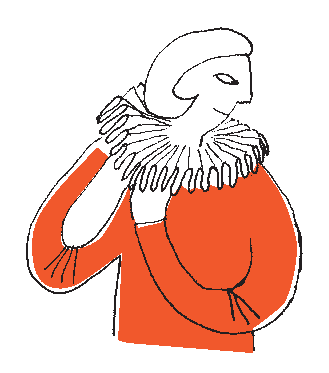
\includegraphics{art/202502_kol05}}
 \vskip2pt

\hbox to\hsize{%
\vbox{\hsize5cm\scriptsize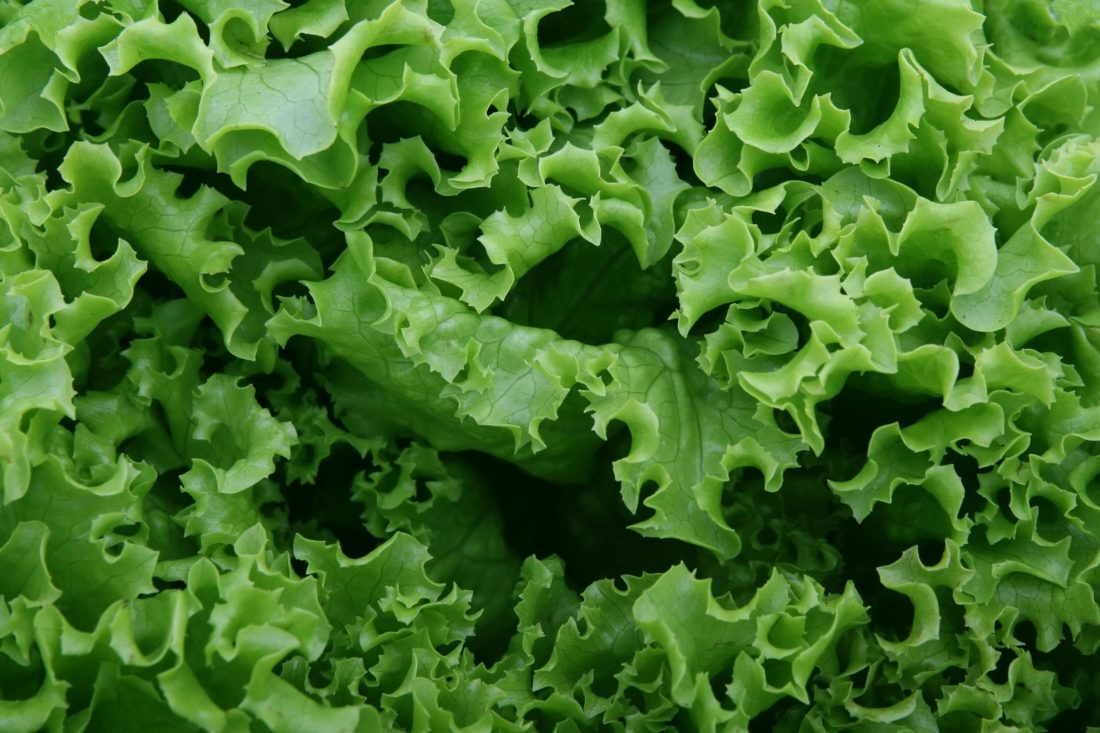
\includegraphics[width=5.5cm]{ilustracje/lettuce.jpg} \\[2mm]
Sałata -- proces jej wzrostu przypomina efekt szydełkowania opisany w~\dlink{https://www.deltami.edu.pl/2020/05/zrob-to-sam-plaszczyzna-hiperboliczna-szydelkiem/}{5}{20}}\hfill
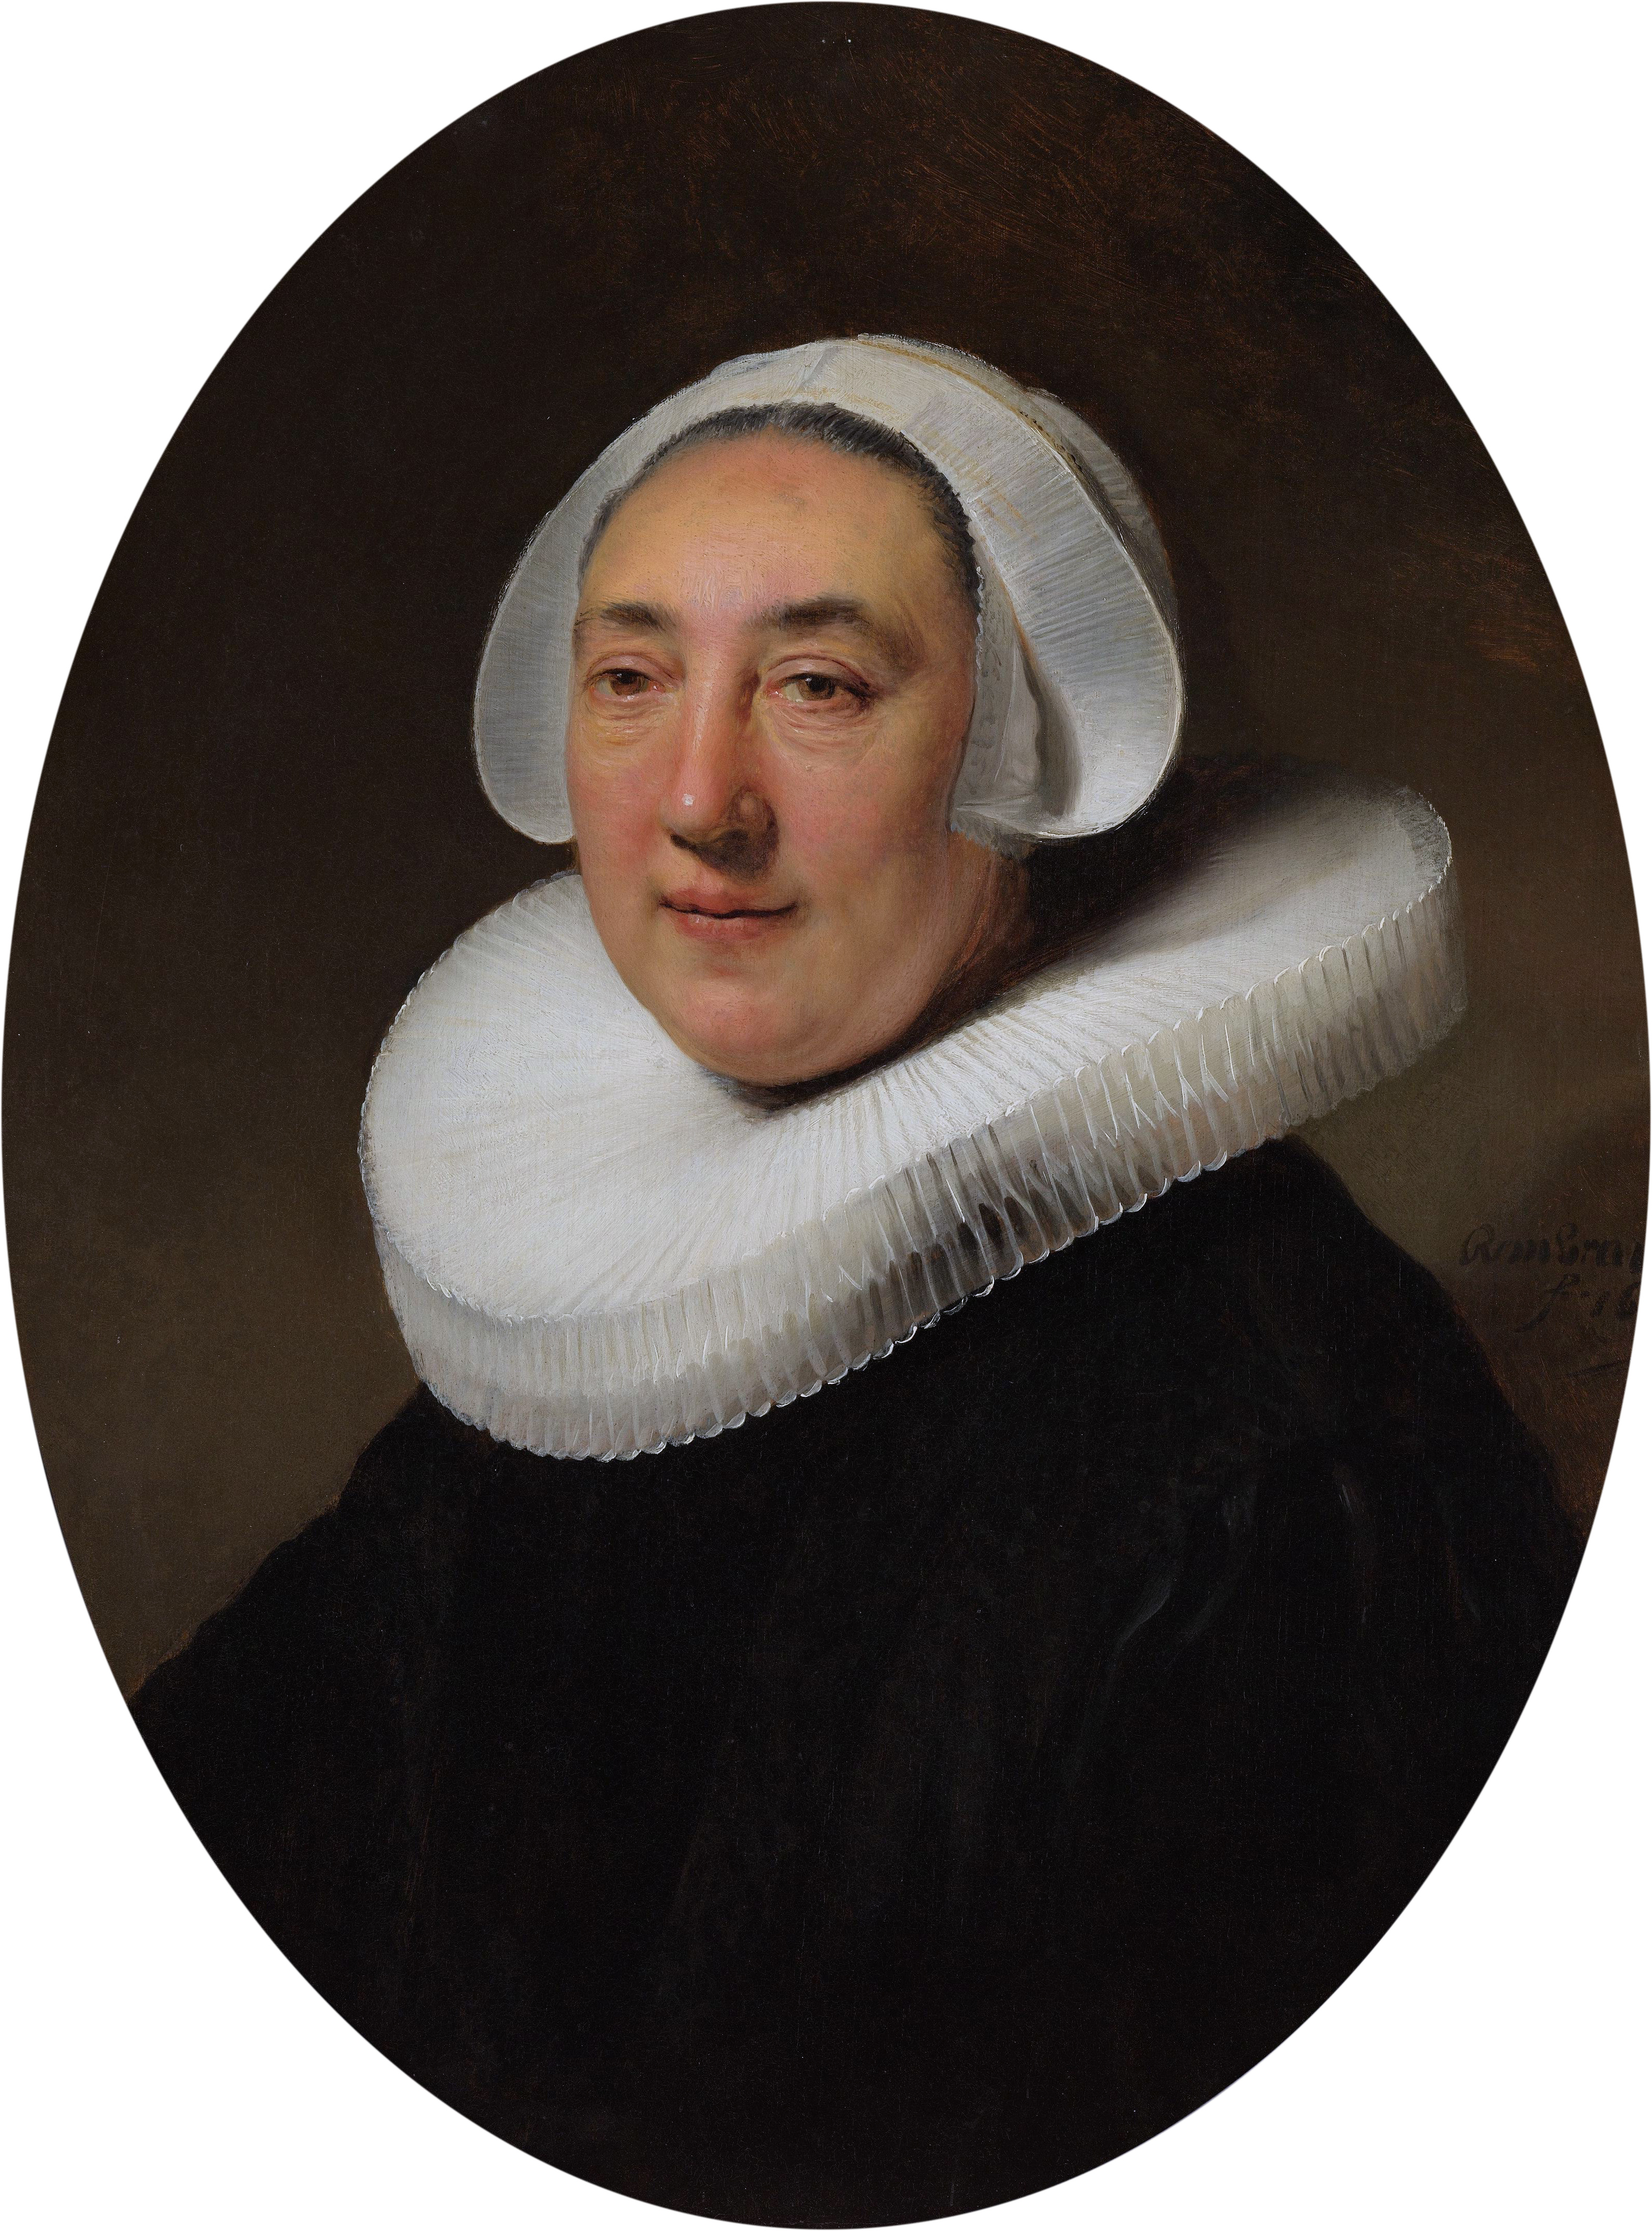
\includegraphics[height=46mm]{ilustracje/Portret_van_Haesje_Jacobsdr_van_Cleyburg.jpg}\quad\vbox{\hsize2.3cm\scriptsize
Portret Haesje~Jacobsdr van~Cleyburg, żony pewnego rotterdamskiego piwowara. \\
Rembrandt van Rijn, 1634 (zbiory Rijksmuseum w~Amsterdamie)
}}\vskip-2pt

Płaszczyznę hiperboliczną odkryli niezależnie J{\'a}nos Bolyai (1802--1860) i~Nikołaj Iwanowicz Łobaczewski (1792--1856) (więcej w~\dlink{https://www.deltami.edu.pl/2018/08/geometria-bolyaia-lobaczewskiego-co-to-jest-i-jak-ja-poznawac/}{8}{18}). Choć nie wynika to bezpośrednio z~dotychczasowych obserwacji, płaszczyzna hiperboliczna posiada dużo więcej symetrii niż tylko obrót wokół wyróżnionego punktu, stąd też jej nazwa sugerująca identyczną geometrię wokół każdego punktu. W~istocie powierzchnia ta ma w~każdym punkcie krzywiznę równą $-1$ 
\marg[-52]{
\textbf{Przykłady} powierzchni o~stałej krzywiźnie: \\
\begin{itemize}[nosep,leftmargin=*]
\item $\mathbf{0:}$ \ $h(s) = s$, płaszczyzna,
\item $\mathbf{R^{-2}:}$ \ $h(s) = R \sin(s/R)$, sfera o~promieniu~$R$,
\item $\mathbf{-R^{-2}:}$ \ $h(s) = R \sinh(s/R)$, przeskalowana płaszczyzna hiperboliczna. 
\end{itemize}
Powyższe funkcje $h$ łączy to, że spełniają równanie różniczkowe $h'' + k \cdot h = 0$ z~warunkami początkowymi $h(0) = 0$, $h'(0) = 1$ (choć dla różnych wartości $k$). Każdą inną powierzchnię o~stałej krzywiźnie da się ,,zbudować'' z~jednej z~powyższych.
}
i~jest to -- w~odpowiednim sensie -- jedyna taka powierzchnia. Jej zobaczenie utrudnia wykazane przez Davida Hilberta (1862--1943) twierdzenie mówiące, że nie tylko nie można jej przedstawić jako powierzchni obrotowej, ale w~ogóle nie da się jej izometrycznie zanurzyć (czyli zrealizować bez deformacji) w~przestrzeni trójwymiarowej. Dlatego też sięganie po opis wewnętrzny jest przy zwiedzaniu dziwnych nowych światów nie tylko ciekawe, ale i~konieczne.\goodbreak

\normalsize